\documentclass[a4paper, 12pt]{article}
\usepackage{templates/sbc-template}
\usepackage{color}
\usepackage{graphicx}
\usepackage[brazil]{babel}
\usepackage[utf8]{inputenc}
\usepackage{epsfig}
\usepackage{float}
\usepackage{graphics}
\usepackage{url}
\usepackage[tight,footnotesize]{subfigure}
\usepackage{stfloats}
\usepackage{enumerate}
% \usepackage[left=3cm,top=3cm,right=3cm,bottom=3cm]{geometry}


% correct bad hyphenation here
\hyphenation{op-tical net-works semi-conduc-tor}


\begin{document}

\title{Arquitetura para Mitigação de Ataques DDoS}

\author{
Cinara Menegazzo\inst{1},
Fernando Cezar Bernardelli\inst{1}, \\
Fernando Henrique Gielow\inst{1},
Nadine Lipa Pari\inst{1}
}
   

   
\address{Departamento de Informática -- Universidade Federal do Paraná\\
NR2 - Núcleo de Redes Sem Fio e Redes Avançadas\\
  Caixa Postal 19.081 -- 81.531-980 -- Curitiba -- PR -- Brasil
  \email{\{cmenegazzo,fcb06,fhgielow,nelpari\}@inf.ufpr.br}
}     

\maketitle


\begin{resumo}
%!TEX root = ../proposta.tex


\end{resumo}



\section{Introdução}
%!TEX root = ./proposta.tex

Diversas pesquisas têm sido desenvolvidas buscando soluções para os problemas da Internet atual, que se propagam para a Internet do Futuro (IF). Tais problemas podem ser amplamente categorizados nas áreas de mobilidade, qualidade de serviço e segurança, os quais ainda caminham para soluções aceitáveis, ajudados pelo surgimento de novas arquiteturas. Hoje tanto os dados quantos as aplicações são disponibilizados em localizações físicas distintas e desconhecidas. Outra grande mudança ocorreu na forma de administrar um sistema, que antes era de âmbito mais local, com seus usuários e servidores característicos, e agora esses sistemas são hospedado em ambientes construídos pelo compartilhamento de recursos de diversos sistemas autônomos (AS), heterogêneos~\cite{5486552}.

O uso massivo dos recursos disponibilizados na Internet e toda a conectividade proporcionada com serviços para uso pessoal, comercial ou acadêmico, torna este ambiente um alvo visado para códigos maliciosos. Ademais, isso é agravado pela forma como a arquitetura TCP/IP pode favorecer um atacante. O protocolo IP (\emph{Internet Protocol}) omite as informações da verdadeira identidade de um emissor, e essa não autenticação da fonte permite que um usuário realize um ataque contra qualquer outro usuário, podendo permanecer anônimo e impune~\cite{1039856}.

Apesar de muitos anos de esforços de pesquisadores, os ataques de \emph{Denial of Service} (DoS) ainda representam sérias ameaças a muitos servidores na Internet.  Ele se configura como um dos principais desafios de segurança atualmente propagado para a IF, que interconecta muito mais dispositivos e indivíduos. O ataque por DoS não visa invadir um computador para obter informações confidenciais, nem tão pouco alterar informações armazenadas nele. Seu objetivo é a indisponibilização de um serviço fornecido, utilizando-se do encaminhamento de grandes quantidades de requisições ao hospedeiro do serviço. Essa questão torna-se ainda mais severa quando diversos geradores de tráfego intensificam essa ação de maneira distribuída, caracterizando um ataque de \emph{Distributed Denial of Service} (DDoS \cite{Sachdeva08ddosincidents}). A consequência desse ataque é o congelamento, a reinicialização, ou ainda o esgotamento completo de recursos alocados para o cliente. Os serviços que mais sofrem com este tipo de ataque são aqueles que permitem requisições anônimas, como os \textit{web}. O desafio de eliminar os ataques de DDoS está na dificuldade de determinar a diferença entre pacotes legítimos e pacotes de atacantes \cite{Li:2009:DDA:1683304.1684620}.

Com as novas arquiteturas de rede e de aplicações que configuram a IF, surgem sistemas complexos e robustos como \emph{Clouds} (Nuvens), onde o desafio de mitigar ataques DoS torna-se ainda mais necessário. A maioria das soluções comumente oferecidas para mitigar DDoS em \emph{cloud} se baseia na maior alocação de recursos \cite{Peng:2007:SND:1216370.1216373}, porém elas também aumentam os custos do usuário para manter tais recursos. Este comportamento carateriza \emph{economic DDoS} (eDDoS) \cite{Soon:10}.  

Algumas abordagens diferenciadas se mostram inadequadas por assumirem premissas que nem sempre são verdadeiras, ou por serem custosas demais \cite{Bakshi:10}, \cite{Liu:2010:NFD:1866835.1866849}. De acordo com estudos recentes, esse tipo de ataque ainda é muito disparado, graças às \textit{botnets}, ou redes zumbi. Um exemplo destas é a rede TDL-4, que é classificada por especialistas em segurança como “não perfeitamente, mas praticamente indestrutível”, com aproximadamente 4,5 milhões de infecções só em 2011 \cite{tdl4}. A partir de fevereiro 2010, o grupo ativista \textit{hacker} conhecido como \textit{Anonymous} começou uma série de ataques de cunho político e ideológico contra várias instituições de porte internacional \cite{titstorm}. A parte mais massiva desses ataques era constituída de DDoS.

A necessidade de proteger as arquiteturas de rede ou de mitigar ataques de DDoS tem sido reconhecida tanto no meio acadêmico quanto comercial. A maioria das soluções de segurança são construídas focadas na prevenção de ataques \cite{4429182}. Contudo, os atuais sistemas em redes são tão complexos que é impossível identificar e corrigir todas as suas vulnerabilidades antes que elas se tornem ataques ou intrusões e, muitas vezes, impossível de se recuperar de falhas decorrentes. Logo, a garantia de funcionamento destes sistemas sob condições de ataques ou intrusões têm se tornado uma prioridade. Diversos autores, como \cite{Verissimo} e \cite{4796927}, têm defendido que as linhas clássicas de defesa não apresentam abordagens que garantam a tolerância a falhas em caso de ataques ou intrusões. Temos então a abordagem de \textbf{tolerância a intrusão}, que garante o funcionamento dos sistemas mesmo que estejam sob ataque, minimizando os prejuízos até o retorno do fluxo normal de funcionamento \cite{Fraga_Powell_1985}. Ao invés de tentar se prevenir de todo tipo de ataque ou intrusão, os sistemas passam a tolerar os problemas simples de segurança e criam mecanismos de controle à intrusão  de forma que eles não causem falhas críticas no sistema. Esta abordagem faz uso de replicação ou redundância para garantir os aspectos de tolerância e são aplicados especificamente quando a forma de intrusão ou ataque seja diferenciada ou desconhecida \cite{4796927}. 

Este trabalho propõe um mecanismo reativo e tolerante a falhas para a mitigação de ataques de DDoS executados contra aplicações hospedadas em uma \emph{cloud}. Tal mecanismo é baseado na instanciação de uma réplica da aplicação - operação simples em uma cloud - e redirecionamento de apenas requisições legítimas à réplica.  Ele monitora o tráfego de uma aplicação, e quando um ataque distribuído de negação de serviço é detectado, cria uma nova instância dessa aplicação, garantindo que nenhum tráfego malicioso a alcance. A solução é inovadora porque não precisa identificar os clientes atacantes e, ainda assim, consegue filtrar apenas o tráfego legítimo sem a carga e possíveis erros de categorização que seriam introduzidos pela tentativa de identificação de clientes. Uma avaliação experimental considerando o tempo de resposta aos clientes, bem como a sobrecarga ao sistema, mostra a eficácia do mecanismo proposto diante de ataques DDoS a um serviço Web.

O restante do artigo está organizado da seguinte maneira: a Seção 2 apresenta os trabalhos relacionados. A Seção 2 detalha a arquitetura do mecanismo proposto para a mitigação de ataques \emph{DDoS}. A Seção 4 apresenta uma descrição da implementação realizada da arquitetura. A Seção 5 apresenta uma avaliação, juntamente com o cenário e os resultados. Por fim, a conclusão e trabalhos futuros são apresentados na Seção 6.



\section{Trabalhos Relacionados}
%!TEX root = ./proposta.tex


As pesquisas que envolvem propostas de mitigação de DDoS em arquiteturas de \emph{cloud}, ainda são consideradas incipientes e distantes de uma convergência. Dentre as poucas propostas para estes ambientes, destaca-se o \emph{framework} pró-ativo CluB, apresentado em \cite{Hazelhurst:2008:SCU:1456659.1456671}, que %considera uma \emph{cloud} como uma rede constituída de um conjunto de \emph{clusters} ou AS. Este trabalho 
sugere
que sejam selecionados determinados roteadores, dispostos de forma distribuída, para análise de tráfego e consequente prevenção de atividade maliciosa. %que as requisições maliciosas alcancem a aplicação. %Estes roteadores são responsáveis por gerar \emph{tokens} de autenticação para legitimar os pacotes, sendo que a autenticação é necessária para a entrada, saída ou trânsito na arquitetura. Cada \emph{cluster} tem seu código de autenticação, que é trocado periodicamente, podendo ser gerado por uma função \emph{hash}, como MD5 ou SHA. O uso de ferramentas apropriadas de criptografia e atualizações periódicas de componentes da infraestrutura fazem parte da proposta do CluB. 
Neste \emph{framework}, todo pacote%, malicioso ou não,
 precisa ser verificado para entrar, sair ou transitar na arquitetura. Cada roteador alocado deverá realizar a verificação, o que é custoso devido ao \emph{overhead} causado pela autenticação de cada pacote e pela necessidade inviável de alterar o comportamento dos roteadores. %Também é necessária a implantação e atualização dos algoritmos de análise de tráfego na arquitetura onde estaria sendo utilizado o CluB. Esta questão se torna inviável ao se tratar de uma \emph{cloud}, devido à nebulosidade de sua arquitetura e infraestrutura.

\cite{Verkaik:2006:PCD:1162666.1162673} apresentam uma proposta pró-ativa, que emprega Comunidades de Interesse (COIs) para capturar dados sobre o comportamento coletivo das entidades remotas, utilizando-os para predizer o comportamento futuro. Tal proposta se baseia no fato de que clientes que tiveram relações legítimas anteriormente possuem bons indícios e podem ser considerados novamente legítimos. %Estas afirmações são geradas da observação de comunicações normais da rede e são utilizadas em conjunto com políticas específicas do servidor para mitigar pró-ativamente os ataques de DDoS, usando mecanismos existentes nos roteadores. 
%
Entretanto, a identificação dos clientes passados não é tão trivial. Além do pequeno \emph{overhead} gerado pela verificação, endereços IPs são normalmente dinâmicos e a exigência da realização de \emph{login} para a identificação não é possível, dado que o ataque de DDoS pode a impossibilitar.


Em \cite{Bakshi:10}, os ataques são tratados através da criação de uma nova instância da aplicação. Uma vez que um ataque DDoS é detectado, a proposta busca identificar os atacantes através de PINGs: caso um cliente suspeito de ser atacante não responda ao PING, ele é considerado como um atacante, de fato. Desta maneira, apenas os clientes que responderem ao PING serão 
redirecionados para a nova instância da aplicação. Entretanto, tal abordagem depende da premissa que atacantes jamais responderão a PINGs e que clientes genuínos sempre responderão, o que nem sempre condiz com a realidade.



% \cite{Walfish:2010:DDO:1731060.1731063} apresenta uma forma de mitigação de ataque classificada como defesa baseada em recursos \cite{Dwork:1992:PVP:646757.705669}.
% Toda vez que um determinado limite de banda é consumido com requisições para um servidor, este servidor, antes que seus recursos se esgotem, encoraja seus clientes a enviar volumes ainda mais altos de tráfego. Considera-se que os atacantes já estariam usando sua capacidade máxima e, assim, eles não poderiam reagir ao encorajamento. A proposta se baseia na premissa que bons clientes têm condições de aumentar seu uso de banda e reagir de forma drástica ao encorajamento. O resultado pretendido é que os bons clientes dominem os maus clientes ao capturar uma fração maior de recursos do servidor. O cliente será atendido caso ele tenha banda o suficiente para se sobressair mediante o tráfego dos atacantes. Um tanto curiosa, esta proposta ocasiona diversos problemas como
% o encorajamento a recebimento de ainda mais tráfego em cenários de ataque. 
% Difícilmente um serviço conseguirá atender a tantas requisições e clientes legítimos não necessariamente dominarão o tráfego que chega ao servidor.


Obviamente, a eficácia de todos os esquemas depende criticamente da capacidade de se identificar ou filtrar os clientes legítimos. 
%
WebSoS \cite{Stavrou:2005:WOS:1090583.1648614} é uma adaptação de \emph{Secure Overlay Services} (SOS) \cite{Keromytis:2002:SSO:964725.633032} que mitiga DDoS em servidores web, reativamente após a detecção do ataque. Com uma filtragem robusta de tráfego e bloqueio de requisições~não aprovadas, forma-se um \emph{overlay} seguro. O servidor utiliza mecanismos de autenticação criptográfica e um teste gráfico de Turing \cite{Dietrich00analyzingdistributed} para diferenciar clientes humanos de \emph{scripts} de ataque. Estes procedimentos, segundo os testes dos autores, não sobrecarregam o funcionamento do serviço, porém exigem que os roteadores localizados no perímetro do servidor sejam configurados para controlar o tráfego, procedimento inviável para arquiteturas de \emph{cloud}.

 



\section{Arquitetura para Mitigação de DDoS em \emph{Cloud}}
%!TEX root = ./proposta3.tex


%Uma estrutura de \emph{cloud} envolve a comunicação entre inúmeros componentes de serviços web. Os usuários desta arquitetura não sabem e não precisam saber sobre a localização de seus dados ou as aplicações que desejem utilizar, porém precisam aceitar e dependem  dos níveis de segurança vigentes, que são tópicos preocupantes para os administradores. %A segurança em \emph{cloud} compreende as áreas de segurança de dados e da rede, segundo \cite{Dhage:2011:IDS:1980022.1980076}. 

% Enquanto um ataque em dados afeta um número restrito de usuários, um ataque na rede pode comprometer diversos usuários simultaneamente. Como ataques de DDos em uma \emph{cloud} compreendem um ataque à segurança em rede, eles são de importância crítica. Com a nova infraestrutura de recursos criada pelas \emph{clouds}, existe a possibilidade de se mover fisicamente uma aplicação para outro endereço quando ela é atacada por DDoS. Com isso, pode-se garantir tolerância à falhas e conservação de recursos despendidos, pois este novo endereço só será conhecido por solicitantes legítimos.

Este trabalho propõe uma arquitetura para mitigar ataques de DDoS em \emph{clouds} de forma autônoma e independente. A arquitetura proposta pode ser utilizada por qualquer aplicação web hospedada em uma \emph{cloud} que, ao sofrer indícios de um ataque DDoS, filtra o tráfego legítimo e encaminha apenas este para uma nova instância da mesma aplicação. 

Esta arquitetura, ilustrada na Figura \ref{fig:arq}, é composta por um módulo geral chamado de Gerenciador de Tráfego (GT), que não se comunica diretamente com a aplicação. Tal módulo possui os submódulos INA, GB, AT e RT. Vale ressaltar que a instância do banco de dados (BD) é exterior às demais instâncias da \emph{cloud}, pelo fato de que este banco de dados também está nas nuvens, e pode ser acessado de qualquer outra instância \emph{cloud}. As operações realizadas pelo módulo GT são divididas em quatro submódulos.
% GF virou GT XXXXX

\begin{figure}[h!]
\centering
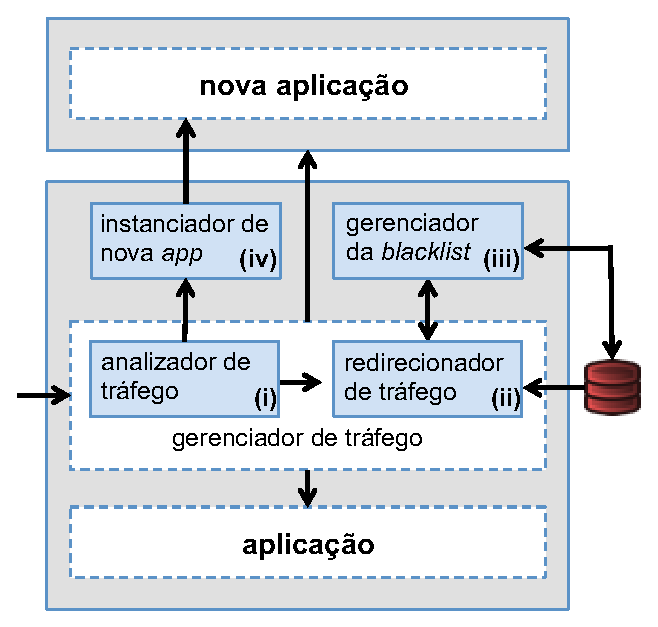
\includegraphics[width=0.45\textwidth]{images/arq.eps}
\caption{Arquitetura para mitigação de ataques DDoS}
\label{fig:arq}
\end{figure}

O submódulo AT observa o comportamento do tráfego de entrada para a aplicação de forma pró-ativa. Focando-se na estimativa de quantidade de tráfego e de processamento no servidor, este submódulo realiza medição para verificar a existência de um possível ataque DDoS. Caso detectado, o submódulo INA é ativado. O INA criará uma nova instância da aplicação em outro servidor na \emph{cloud}, consequentemente com um endereço IP diferente. %\footnote{Com a criação da nova instância da aplicação, a antiga é desativada. A primeira instância da \emph{cloud} servirá apenas para redirecionar o tráfego}.
Com isso, o submódulo RT passará a tratar todo o tráfego de entrada, respondendo com um redirecionamento para a nova instância da aplicação. Parte-se do princípio que atacantes DDoS não interpretam as respostas obtidas do servidor, pois se interpretarem, sua eficiência é reduzida. Desta maneira, apenas os clientes legítimos serão, de fato, redirecionados à nova aplicação.

Ao redirecionar algum cliente para a nova instância, o endereço deste cliente, seja ele legítimo ou não, será adicionado em uma \emph{blacklist}. Os clientes presentes nesta lista têm suas requisições descartadas, a fim de reduzir o custo de processamento de respostas no servidor. Entretanto, como o cliente legítimo é informado antes de seu endereço entrar nesta \emph{blacklist}, isso não será um problema, pois ele já terá acesso à nova instância enviando nova requisição. Entradas com tempo de validade são empregadas nesta \emph{blacklist}, dado que respostas podem ser perdidas. O tempo de validade na lista aumentará exponencialmente, para diminuir ainda mais a sobrecarga. Cabe ao GB, o papel de adicionar e gerenciar a saída de endereços de clientes à \emph{blacklist}, assim como, o tempo de validade da entrada que aumenta exponencialmente.

% Contudo, para prevenir que este controle impeça o acesso de clientes legítimos nas próximas requisições, o cliente, ao ser direcionado para a nova instância, terá este endereço armazenado na forma de \emph{cookies} em sua máquina. Este procedimento garante que apenas clientes legítimos tenham conhecimento do novo endereço da aplicação, dado que atacantes de DDoS não irão manter \emph{cookies}. Por fim,  tal processo de reinstanciação de aplicação e redirecionamento de tráfego pode ser repetido recursivamente, até um dado número máximo de redirecionamentos.

% A Figura~\ref{fig:cen} ilustra um cenário sob ataque de DDoS, sendo que os clientes são representados pelos ícones dos diversos navegadores, e a nave é o logo da aplicação LOIC (\emph{Low Orbit Ion Cannon}). À esquerda, todos eles enviam seu tráfego para o que imaginam ser a instância da aplicação. Considerando um cenário sob ataque, a aplicação será replicada, e a sua instância original servirá para redirecionar o tráfego legítimo até a aplicação nova. À direita, é ilustrado o resultado do redirecionamento: clientes genuínos conseguem atingir a instância nova da aplicação, enquanto os atacantes mantém o ataque na antiga instância de \emph{cloud}, que agora opera apenas redirecionando tráfego.
% 
% 
% \begin{figure}[t!]
% 	\centering
% 	\includegraphics[width=0.40\textwidth]{images/an1.eps}
% 	% \caption{bla}
% 	\hskip 1cm
% 	\includegraphics[width=0.40\textwidth]{images/an2.eps}
% 	\caption{Comportamento do tráfego em um cenário sob ataque}
% 	\label{fig:cen}
% \end{figure}



\section{Implementação}

% \subsection{Detecção de DDoS}
% %!TEX root = ./proposta3.tex


% \subsection{Mecanismo de mitigação}
For the implementation, initially the possibilities for Cloud Servers were taken in account, like Amazon, Linode and Heroku. Among those, the one shown best fit for the practical implementation of an operational prototype of our mechanism was Heroku. \cite{heroku} is a Cloud solution which offers the infrastructure to the hosting service we need. It also allows the use of frameworks like Django, Ruby on Rails (RoR) and node.js. Between the alternatives, we chose the RoR solution, due to the fact that we have greater experience in this technology, but our mechanism is not framework or language dependent, an as such, our experiment could be reproduced in any other alternative of language and framework.

The architecture of the RoR Framework in completely based on the Model View Controller (MVC) paradigm, making it easier to organize the modules in our mechanism. This way, the code structure is composed by parts of Model, View and Control. The \textbf{Model} part concerns everything related to the data -- how it is stored, fetched and related. The \textbf{View} part is related to any graphics the application may show. Least, \textbf{Controllers} handle data, they concern the logical and functional part of the code. They also make the bridge between Model and View, allowing the data to transit in both ways.

Thus, the Traffic Analyzer (TA) submodule of the mechanism belongs to the Controller part. A request to the application will be intercepted by this component, which will probe some statistic data, and soon after, will call the controller responsible by the functioning of the application itself. It is important to notice, however, that time spent in this controller is undermost, only the necessary to process a few equations and store the results for statistical control. Just in case this process may affect the functioning of the application, it might be performed in background.

Case the TA detects the existence of a possible attack, a new instance of the application in the Cloud is created by the NAI submodule, paralyzing the original application, that becomes just a traffic redirector. The re-instantiantion process for an application may happen in two ways. The most simple approach would be that the second application already exists, but with no allocated resources. However, this approach does not behave in the best way possible for a recursive scenario of re-instantiation. The second approach concerns hosting the project in a GitHub repository, so it may be cloned into the second instance via ruby code.

One interesting particularity of the RoR framework is the existence of a routes configuration file. The implementation of the TR submodule will be made using this file, called \textit{routes.rb}. In order to show any dynamic page from the application, this file is inevitably requested. Thus, that is the ideal place to add clients to a blacklist and filter clients blocked by the BM. When redirecting traffic to a new instance, a new entry should be added, blocking the client who sent the request for a certain time.

The blacklist itself and many others control variables will be managed by the database in the \emph{Cloud}~\cite{redis}. Such database if famous by its simplicity and efficiency. It basically maps \textbf{key} and \textbf{value}, offering reading and writing time equivalent to a hash. This way, one option to implement the blacklist in Redis is using the client's IP as a key, and the time it will be blocked is the value mapped by it. The time to check a client is O(1), for it is, abstractly, a hash, and this is excellent for a mechanism that will filter all the incoming traffic. A structured view of the functions performed by the proposed architecture is described in the flux diagram illustrated in the figure~\ref{fig:dfd}.

\begin{figure}[t!]
	\centering
	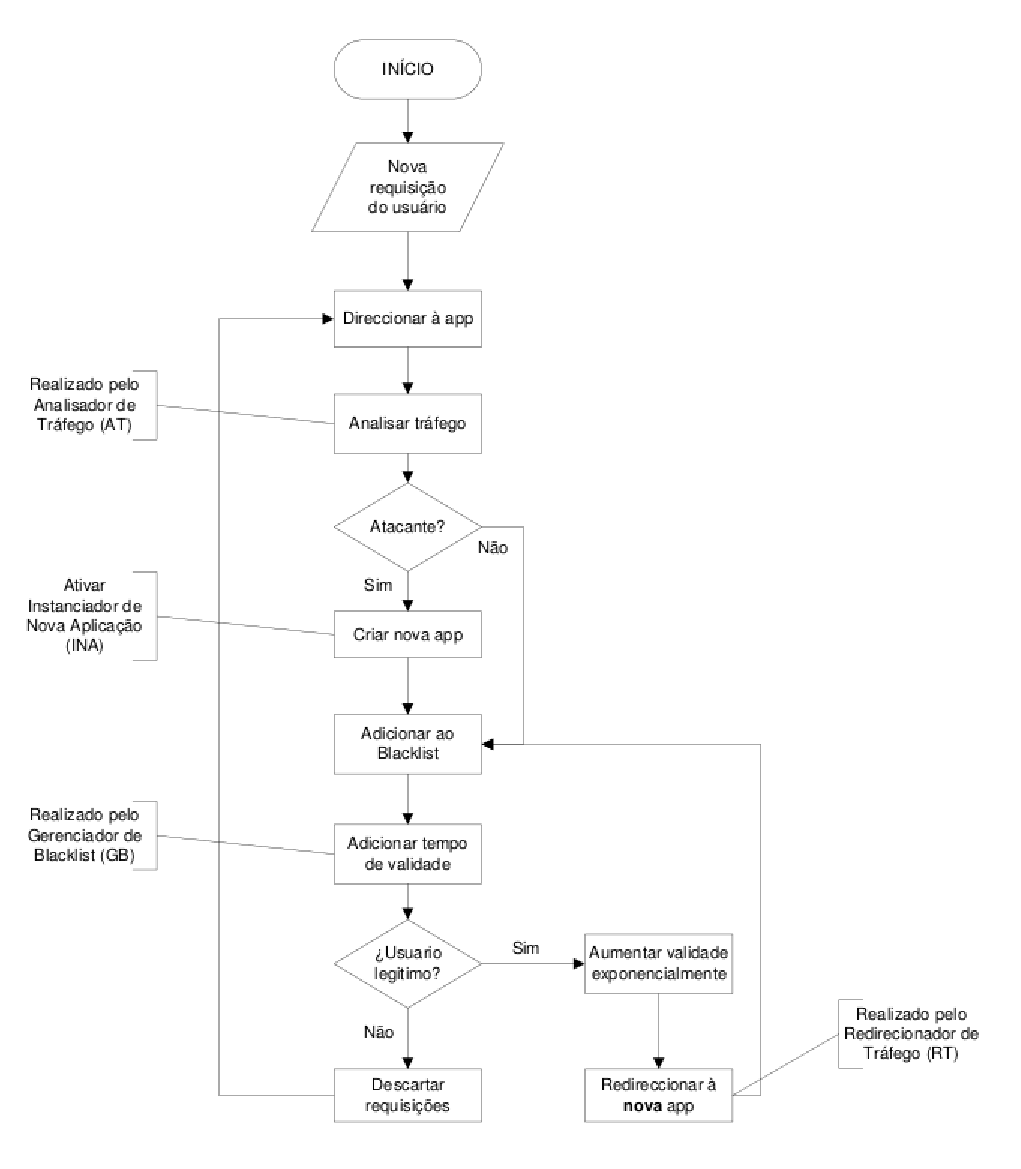
\includegraphics[width=0.90\textwidth]{images/dfd.eps}
	\hskip 1cm
	\caption{Functions of the DDoS mitigating architecture}
	\label{fig:dfd}
\end{figure}

Least, an interesting feature of using Heroku are the many add-ons it offers. I particular, there is one add-on called New Relic which is responsible for collecting data for performance analysis. This add-on will make it possible to know precisely what is going on in every instance of the application in a Cloud from a internal perspective. Thus, we will be able to probe data of not only the external perspective (which is the user perspective), but also the internal view.

\section{Descrição da Avaliação}
%!TEX root = ./proposta3.tex


%A avaliação de um sistema de defesa para ataques pode ser avaliado sobre os aspectos de sua construção. 
% WTF esse trecho acima? xD
%
Uma solução para mitigar ataques pode ser avaliada quanto a sua capacidade de detectar ataque, assim como, a de reagir a ele. Outra abordagem para avaliar uma solução é quanto a sua capacidade de manter as condições normais de funcionamento do cenário de ataque, mesmo sob ataque. Segundo \cite{4600003} é importante para um sistema de defesa estimar diversos aspectos como: custo de desenvolvimento, desempenho, degradação do serviço e custo de robustez. 

A maioria das métricas para calcular o impacto de ataques DDoS estão relacionadas com as medidas de eficiência dos padrões de defesa \cite{4809152}. Atualmente, são consideradas estratégias de medição da quantidade de tráfego legítimo que chega até a aplicação. Outros trabalhos tem se concentrado na medida do tempo de resposta para avaliar a eficiência de uma solução. \cite{Mirkovic:2007:TUM:1281700.1281708} utiliza um modelo baseado em \emph{threshold} como métrica para aferir o impacto de DDoS. Quando uma medida excede este \emph{threshold}, ocorre a  indicação da baixa qualidade do serviço. Esta medida é indicada para aplicações fim-a-fim, como o HTTP.

\textbf{Arrumar verificar se foram estas levantadas nos gráficos}
A etapa de avaliação do nosso mecanismo consistirá principalmente na análise
da capacidade do servidor em atender novas requisições. Se o ataque de DDoS for devidamente
mitigado, as requisições de atacantes serão ignoradas, após a inclusão do requisitante na \emph{blacklist}. Assim, o servidor na \emph{cloud} deverá ser capaz de redirecionar apenas clientes legítimos 
para a nova instância e garantirá que eles terão acesso direto nas próximas requisições. 
Portanto, de acordo com as métricas especificadas por \cite{4600003}, este trabalho de pesquisa foi avaliado pelo uso de métricas como o tempo de resposta do servidor para requisições atendidas, a taxa de requisições atendidas com relação ao número de clientes, a carga gerada pelos módulos da arquitetura de acordo com o número de clientes \footnote{O termo ``clientes'', usado neste parágrafo engloba tanto clientes legítimos quanto atacantes.}. 

Cabe ressaltar que este trabalho não necessita de uma previsão muito grande na detecção do tipo de ataque, no sentido de que é melhor realizar uma calibragem muito sensível e possuir falsos positivos do que possuir falsos negativos, isto se deve à natureza do mecanismo implementado. Se uma nova instância for criada e o tráfego for redirecionado à toa, o custo será de apenas alguns mínimos milisegundos de latência. Caso o mecanismo não detecte um ataque, o custo será muito mais significativo. Desta maneira, a avaliação quanto à falsos positivos não é crucial. % quanto a avaliação não detecção do ataque. 


\subsection{Cenários}
%!TEX root = ./proposta3.tex

% Para a simulação do tráfego necessário, podem ser utilizadas ferramentas que enviam requisições HTTP à aplicação. Como ferramentas, podem ser citados os comandos \emph{curl} e \emph{ab} e a aplicação \emph{LOIC}. A diferença fundamental dentre elas é o nível na qual operam. Enquanto o comando \textbf{curl} opera realizando instâncias singulares de operações simples como \emph{GET}s e \emph{PUT}s, o comando \textbf{ab} automatiza o processo realizando diversas operações de acordo com alguns parâmetros. É possível customizar o nível de concorrência e o intervalo entre as requisições, por exemplo. Tal ferramenta possibilita a medição de algumas métricas como a taxa de entrega de pacotes e o tempo de resposta. Em um nível ainda maior, a aplicação~\cite{loic} foi desenvolvida a fim de realizar ataques de DoS\footnote{Diversos clientes a utilizam a fim de gerar um ataque de DDoS.}. %Ela realiza automaticamente a calibragem de diversos parâmetros em níveis inferiores. Entretanto, ela ainda permite a customização de alguns, como a porta de ataque e o protocolo a ser utilizado.

% Considerando estas ferramentas, um cenário foi elaborados para a avaliação. 
%
% Para a simulação de clientes, o comando \emph{curl} foi utilizado para criar um \emph{script} que atua como um cliente legítimo ou atacante. O comando requisita a página em questão através de um \emph{GET}. Caso a resposta indique uma mudança de endereço, o \emph{script} é responsável por seguir todas as mudanças e redirecionamentos com chamadas subsequentes do comando \emph{curl}, até que o destino final seja de fato atingido. Deve-se ressaltar que esse comportamento é dificultado em atacante de DDoS, pois eles perderiam muito a sua eficiência ao aguardar por respostas de requisições, analisá-las, e seguir até o destino final.

Para a experimentação, como nós maliciosos, foram utilizadas 8 máquina do laboratório de pesquisas NR2 para processar os ataques, observando-se uma latência de rede no intervalo de $3ms$ a $7ms$. Cada uma destas máquinas operou com 25, 50, 75 ou 100 instâncias de um \emph{script} atacante, que utiliza o comando \emph{curl} para bombardear o servidor com requisições HTTP do tipo \emph{GET}. %As ferramentas \emph{LOIC} e \emph{ab} não foram utilizadas por se mostrarem inadequadas. Enquanto o \emph{LOIC} não permitia o uso do endereço da aplicação hospedada como alvo do ataque, a ferramenta \emph{ab} não opera da maneira esperada, criando padrões de tráfego fora das necessidades para este projeto.
%Para a obtenção de tempos de resposta e taxa de perda de pacotes da perspectiva do cliente, o comando \emph{ab} pode ser empregado para realizar as medições. Diversas faixas de parâmetros podem ser estipuladas para simular diferentes tipos de comportamentos ou cenários. O uso do \emph{ab} torna-se preferível ao do \emph{curl} quando o objetivo é coletar métricas e não simular um cliente genuíno, afinal, o comando \emph{ab} medirá o desempenho de instâncias \emph{cloud} isoladas, sem realizar qualquer redirecionamento de tráfego. Este aspecto do comportamento do \emph{script} em questão é importante para a diferenciação entre ataques DDoS e \emph{Flash Crowds}~\cite{Thapngam:2011p27061}. Enquanto um ataque é malicioso, uma \emph{Flash Crowd} indica que diversos clientes legítimos estão, de fato, realizando diversas requisições à aplicação. Este caso não será tratado, embora talvez pudesse ser identificado.

%\textbf{justificar o nao uso do LOIC e colocar o cenário}
% Por fim, para a simulação do ataque DDoS em si, a ferramenta \emph{LOIC} pode ser utilizada, pois ela é uma ferramenta para ataques reais. Embora a escala em nosso experimento seja muito menor, a operação será baseada em um ataque real e, portanto, condizente com a realidade. Para a obtenção de diferentes endereços IP, diferenciando um DoS de um DDoS, a ferramenta será utilizada simultaneamente por computadores de endereços diferentes.
% No cenário de simulação foram utilizados oito nós atacantes executando \emph{scripts} de ataques simultâneos, originando 25, 50, 75 e 100 processos atacantes sobre uma latência de 3 a 7 milisegundos.



\subsection{Resultados}
\input{parts/a07-cenarios}

\section{Conclusão}
\input{parts/a08-conclusao}


%\section{Cronograma}
%%!TEX root = ./proposta3.tex

O desenvolvimento deste trabalho de pesquisa segue as etapas descritas no cronograma descrito abaixo, onde '$\circ$' define as atividades já realizadas e '$\bullet$' as atividades a serem desenvolvidas 
{\footnotesize
\center
\begin{table}[ht!]
\footnotesize
\center
\begin{tabular}{|c||c|c|c|c|c|c|c|}
\hline

      & \textbf{Nov/1} & \textbf{Nov/2} & \textbf{Nov/3} & \textbf{Nov/4} & \textbf{Dez/1} & \textbf{Dez/2} & \textbf{Dez/3} \\
\hline
\hline
Elaboração da proposta de solução      &  {$\circ$} & {$\circ$} &  &  &  &  &  \\
\hline						
%&  {\color{green}$\bullet$} & {\color{green}$\bullet$} &  &  &  &  &  \\
Estudo de métricas de desempenho      &  & {$\circ$} & $\bullet$ &  &  & &  \\
\hline									

Pesquisa sobre detecção de DDoS      &  & {$\circ$} & $\bullet$  &  &  &  &  \\
\hline									


Pesquisa sobre ferramentas       &  &  & {$\circ$} &  &  &  &  \\
para geração de requisições       &   &   &   &   &   &   &   \\
\hline									


Implementação dos módulos      &  &  &  {$\circ$} & $\bullet$ & $\bullet$ & $\bullet$ &  \\
\hline									

Escrita do relatório final      &  &   & {$\circ$} & $\bullet$  & $\bullet$ &  $\bullet$ &  \\
\hline

Experimentação      &  &  &  &  &$\bullet$  & $\bullet$ &  \\
\hline
\end{tabular}
\label{tab:crono}
\end{table}
}


\section{Acknowledgements}
%!TEX root = ./proposta3.tex

Este trabalho foi realizado mediante a colaboração de todos os membros da equipe, onde o problema a ser tratado e o escopo de solução foram discutidos por todos e todos tiveram participação. As etapas descritas no cronograma tiveram a seguinte divisão de trabalho, embora a participação de todos seja essencial e deva ser mantida para que o trabalho tenha um todo como resultado e não apenas partes de esforços.


\begin{itemize}
\item Elaboração da proposta de solução - Todos
\item Estudo de métricas de desempenho - Cinara e Fernando Gielow
\item Pesquisa sobre detecção de DDoS - Cinara
\item Pesquisa sobre ferramentas para geração de requisições - Fernando Cezar
\item Implementação dos módulos - Fernando Gielow e Fernando Cezar
\begin{itemize}
\item Especificação de Algoritmos - Cinara e Nadine com suporte de todos
\item Estudo de ferramentas - Fernando Gielow e Fernando Cezar
\end{itemize}
\item Escrita do relatório final - Cinara e Nadine
\item Experimentação - Todos
\begin{itemize}
\item Categorização e medição de métricas - Cinara e Fernando Gielow
\end{itemize}

\end{itemize}





% \newpage
% \bibliographystyle{unsrt}

\bibliographystyle{templates/sbc}
\bibliography{parts/proposta}
\end{document}
